\begin{figure}[htbp]
			\centering
			\resizebox{\textwidth}{!}{%
				\begin{tikzpicture}[
					scale=0.95,
					>=latex,
					trave/.style={line width=1.4pt},
					carico/.style={black, line width=0.6pt},
					forza/.style={black, line width=0.7pt},
					diagT/.style={black, line width=0.8pt},
					diagM/.style={black, line width=0.8pt},
					hatch/.style={gray!50, line width=0.3pt},
					quota/.style={black, line width=0.2pt},
					fibre/.style={gray!70, line width=0.3pt},
					]
					
					% ── Parametri dei vincoli (convenzione C06/C07) ──
					\def\tw{0.15}    \def\thR{0.28}   \def\rn{0.06}
					\def\rw{0.05}    \def\bw{0.09}    \def\gw{0.22}
					\def\hh{0.10}
					
					% ── Geometria del problema ──
					\def\Lell{4}                            % lunghezza trave ℓ
					\pgfmathsetmacro{\xA}{0}
					\pgfmathsetmacro{\xC}{\Lell/3}          % C a ℓ/3 da A ≈ 1.333
					\def\yqi{-0.80}                         % y delle quote sotto la trave
					\def\ylab{-3.30}                        % y delle etichette di pannello
					
					% ── Centri di tratto utili per le etichette ──
					\pgfmathsetmacro{\xMidAC}{0.5*\xC}      % centro tratto AC
					
					% ── Parametri del simbolo "coppia concentrata" ──
					\def\rCoppia{0.25}    % raggio dell'arco
					\def\Lwing{0.12}      % lunghezza dell'ala della freccia
					\def\Lstem{0.05}      % lunghezza del tratto rettilineo (stelo) dal sud dell'arco al punto C
					
					% =========================================================
					% PANNELLO (a) — Schema statico
					% =========================================================
					\begin{scope}[xshift=0cm]
						
						% ── Trave ──
						\draw[trave] (0,0) -- (\Lell,0);
						
						% ── Fibra inferiore (tratteggio sotto la trave) ──
						\draw[fibre, dashed] (0, -0.1) -- (\Lell, -0.1);
						
						% ── Cerniera in A ──
						\draw[thick] (0,0) -- (-\tw,-\thR) -- (\tw,-\thR) -- cycle;
						\draw[thick] (-\gw,-\thR) -- (\gw,-\thR);
						\foreach \x in {-0.16,-0.08,0,0.08,0.16}
						\draw[thin] (\x,-\thR) -- ++(-0.07,-\hh);
						
						% ── Carrello verticale in B ──
						\draw[thick] (\Lell,0) -- (\Lell-\tw,-\thR) -- (\Lell+\tw,-\thR) -- cycle;
						\draw[thick] (\Lell-\bw,-\thR-\rw-0.01) circle (\rw);
						\draw[thick] (\Lell+\bw,-\thR-\rw-0.01) circle (\rw);
						\draw[thick] (\Lell-\gw,-\thR-2*\rw-0.04) -- (\Lell+\gw,-\thR-2*\rw-0.04);
						\foreach \x in {-0.16,-0.08,0,0.08,0.16}
						\draw[thin] (\Lell+\x,-\thR-2*\rw-0.04) -- ++(-0.07,-\hh);
						
						% ── Anellini bianchi sui perni ──
						\draw[thick, fill=white] (0,0) circle (\rn);
						\draw[thick, fill=white] (\Lell,0) circle (\rn);
						
						% ── Etichette A, B ──
						\node[above left=-2pt,  font=\small] at (0,0)      {$A$};
						\node[above right=-2pt, font=\small] at (\Lell,0)  {$B$};
						
						
						% ── Stelo verticale: dal punto sud del semicerchio al punto C sulla trave ──
						\draw[forza] (\xC, -\rCoppia) -- (\xC, 0);
						
						% ── Coppia antioraria μ in C ──
						\draw[forza]
						(\xC, -\rCoppia)
						arc[start angle=-90, end angle=90, radius=\rCoppia];
						% Punta della freccia all'estremità superiore: punta verso sinistra
						\pgfmathsetmacro{\tipxC}{\xC}
						\pgfmathsetmacro{\tipyC}{\rCoppia}
						\draw[forza] (\tipxC, \tipyC)
						-- ({\tipxC + \Lwing*cos(25)},  {\tipyC + \Lwing*sin(25)});
						\draw[forza] (\tipxC, \tipyC)
						-- ({\tipxC + \Lwing*cos(-25)}, {\tipyC + \Lwing*sin(-25)});
						% Etichetta μ in alto a sinistra del simbolo
						\node[left, font=\small] at (\xC - 0.05, \rCoppia) {$\mu$};
						
						% ── Quote ℓ/3 (da A a C) e 2ℓ/3 (da C a B) sotto la trave ──
						\draw[<->, quota] (0,\yqi)   -- (\xC,\yqi);
						\draw[<->, quota] (\xC,\yqi) -- (\Lell,\yqi);
						\draw[quota] (0,\yqi+0.07)     -- (0,\yqi-0.07);
						\draw[quota] (\xC,\yqi+0.07)   -- (\xC,\yqi-0.07);
						\draw[quota] (\Lell,\yqi+0.07) -- (\Lell,\yqi-0.07);
						\pgfmathsetmacro{\xMidCB}{0.5*(\xC+\Lell)}    % centro del tratto CB
						\node[above, font=\footnotesize] at (\xMidAC, \yqi-0.1) {$\ell/3$};
						\node[above, font=\footnotesize] at (\xMidCB, \yqi-0.1) {$2\ell/3$};
						
						% Etichetta pannello (a)
						\node[font=\small] at (0.5*\Lell, 0.4*\ylab) {(a)};
						
					\end{scope}
					
					% =========================================================
					% PANNELLO (b) — Diagramma di T(z)
					% =========================================================
					\begin{scope}[xshift=5.5cm]
						
						% ── Trave (clone) ──
						\draw[trave] (0,0) -- (\Lell,0);
						
						% ── Vincoli (clone) ──
						\draw[thick] (0,0) -- (-\tw,-\thR) -- (\tw,-\thR) -- cycle;
						\draw[thick] (-\gw,-\thR) -- (\gw,-\thR);
						\foreach \x in {-0.16,-0.08,0,0.08,0.16}
						\draw[thin] (\x,-\thR) -- ++(-0.07,-\hh);
						\draw[thick] (\Lell,0) -- (\Lell-\tw,-\thR) -- (\Lell+\tw,-\thR) -- cycle;
						\draw[thick] (\Lell-\bw,-\thR-\rw-0.01) circle (\rw);
						\draw[thick] (\Lell+\bw,-\thR-\rw-0.01) circle (\rw);
						\draw[thick] (\Lell-\gw,-\thR-2*\rw-0.04) -- (\Lell+\gw,-\thR-2*\rw-0.04);
						\foreach \x in {-0.16,-0.08,0,0.08,0.16}
						\draw[thin] (\Lell+\x,-\thR-2*\rw-0.04) -- ++(-0.07,-\hh);
						\draw[thick, fill=white] (0,0) circle (\rn);
						\draw[thick, fill=white] (\Lell,0) circle (\rn);
						
						% ── Etichette A, B ──
						\node[above left=-2pt,  font=\small] at (0,0)      {$A$};
						\node[above right=-2pt, font=\small] at (\Lell,0)  {$B$};
						
						% ── Tacca verticale in C ──
						\draw[forza] (\xC, -0.10) -- (\xC, 0.10);
						
						% ── Diagramma T(z) ──
						\def\sT{2.5}
						\pgfmathsetmacro{\Tval}{(1/\Lell)*\sT}    % T(z) = μ/ℓ = 1/ℓ → 0.25·2.0 = 0.50
						
						% Hatching verticale uniforme su tutta la trave
						\foreach \x in {0.10, 0.30, ..., 3.90} {
							\draw[hatch] (\x, 0) -- (\x, \Tval);
						}
						
						% Bordo del diagramma — rettangolo
						\draw[diagT]
						(0, 0) -- (0, \Tval)             % verticale in A
						-- (\Lell, \Tval)                % uniforme su tutta la trave
						-- (\Lell, 0);                   % verticale di chiusura in B
						
						% Segno cerchiato al centro del rettangolo
						\node[font=\small] at (0.5*\Lell, {0.5*\Tval})
						{$\boldsymbol{\oplus}$};
						
						% Etichetta del valore μ/ℓ sopra il rettangolo, a destra
						\node[above, font=\small] at (\Lell-0.30, \Tval) {$\tfrac{\mu}{\ell}$};
						
						% Etichetta pannello (b)
						\node[font=\small] at (0.5*\Lell, 0.4*\ylab) {(b)};
						
					\end{scope}
					
					% =========================================================
					% PANNELLO (c) — Diagramma di M(z)
					% =========================================================
					\begin{scope}[xshift=11.0cm]
						
						% ── Trave (clone) ──
						\draw[trave] (0,0) -- (\Lell,0);
						
						% ── Vincoli (clone) ──
						\draw[thick] (0,0) -- (-\tw,-\thR) -- (\tw,-\thR) -- cycle;
						\draw[thick] (-\gw,-\thR) -- (\gw,-\thR);
						\foreach \x in {-0.16,-0.08,0,0.08,0.16}
						\draw[thin] (\x,-\thR) -- ++(-0.07,-\hh);
						\draw[thick] (\Lell,0) -- (\Lell-\tw,-\thR) -- (\Lell+\tw,-\thR) -- cycle;
						\draw[thick] (\Lell-\bw,-\thR-\rw-0.01) circle (\rw);
						\draw[thick] (\Lell+\bw,-\thR-\rw-0.01) circle (\rw);
						\draw[thick] (\Lell-\gw,-\thR-2*\rw-0.04) -- (\Lell+\gw,-\thR-2*\rw-0.04);
						\foreach \x in {-0.16,-0.08,0,0.08,0.16}
						\draw[thin] (\Lell+\x,-\thR-2*\rw-0.04) -- ++(-0.07,-\hh);
						\draw[thick, fill=white] (0,0) circle (\rn);
						\draw[thick, fill=white] (\Lell,0) circle (\rn);
						
						% ── Etichette A, B ──
						\node[above left=-2pt,  font=\small] at (0,0)      {$A$};
						\node[above right=-2pt, font=\small] at (\Lell,0)  {$B$};
						
						% ── Tacca verticale in C ──
						\draw[forza] (\xC, -0.10) -- (\xC, 0.10);
						
						% ── Diagramma M(z) ──
						\def\sM{1.4}
						\pgfmathsetmacro{\McMinus}{-(1/3)*\sM}    % M(C⁻) = +μ/3 → sotto: -0.40
						\pgfmathsetmacro{\McPlus}{ (2/3)*\sM}     % M(C⁺) = -2μ/3 → sopra: +0.80
						
						% Hatching tratto AC: lineare, sotto l'asse (M>0)
						\foreach \x in {0.10, 0.30, ..., 1.30} {
							\pgfmathsetmacro{\h}{\McMinus*\x/\xC}
							\draw[hatch] (\x, 0) -- (\x, \h);
						}
						% Hatching tratto CB: lineare, sopra l'asse (M<0)
						\foreach \x in {1.50, 1.70, ..., 3.90} {
							\pgfmathsetmacro{\h}{\McPlus*(\Lell-\x)/(\Lell-\xC)}
							\draw[hatch] (\x, 0) -- (\x, \h);
						}
						
						% Bordo del diagramma — due segmenti lineari + salto verticale in C
						\draw[diagM]
						(0, 0) -- (\xC, \McMinus)         % retta da A a C⁻ (sotto)
						-- (\xC, \McPlus)                 % salto verticale in C (attraversa l'asse)
						-- (\Lell, 0);                    % retta da C⁺ a B (sopra)
						
						% Etichette dei valori notevoli
						\node[right, font=\small] at (\xC, \McMinus-0.04)	{$\tfrac{\mu}{3}$};
						% 2μ/3 sopra il vertice in C⁺ (lobo negativo, sopra l'asse)
						\node[left, font=\small] at (\xC, \McPlus+0.04){$\tfrac{2\mu}{3}$};
						
						% Etichetta pannello (c)
						\node[font=\small] at (0.5*\Lell, 0.4*\ylab) {(c)};
						
					\end{scope}
					
				\end{tikzpicture}
			}
			\caption{Trave appoggiata con coppia concentrata antioraria $\mu$
				applicata in $C$ a distanza $\ell/3$ da $A$:
				(a)~schema strutturale;
				(b)~diagramma del taglio $T(z)$, uniforme pari a $\mu/\ell$
				su tutta la trave (la coppia concentrata non produce salto
				del taglio);
				(c)~diagramma del momento flettente $M(z)$, lineare crescente
				a tratti, da $0$ a $\mu/3$ in $AC$ e da $-2\mu/3$ a $0$
				in $CB$, con salto $-\mu$ in $C$.}
			\label{fig:stat_trasv_iso_08}
		\end{figure}
